\section{Realisation}
\label{realisation}

Our implementation of the plug-in corresponds to the schema presented in the Figure \ref{flowchart}. We can divide our work into 2 stages; first we analyse and model the Android Intents and then develop this model into abstract and concrete syntax. The second stage is the plug-in development where we transform our existing abstract syntax data into structured JDT methods which will be called to perform our code generation. All the steps will be described in more details in this section.  

\begin{figure}[H]
\label{flowchart}
  \centering
    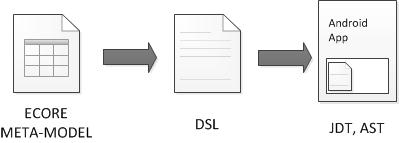
\includegraphics[width=0.8\textwidth]{flowchart}
  \caption{Flow chart}
\end{figure}

We started our project by determining the DSL of Android Intents and built our Ecore meta-model which reflected the DSL. Our DSL was based on several examples taken from Open Intents website\footnote{http://www.openintents.org/en/}, the default Android Intents included in Android, and finally the knowledge presented in the chapter \ref{intents}. The final Ecore model in shown the figure \ref{meta-model}.

\begin{figure}[H]
\label{meta-model}
  \centering
    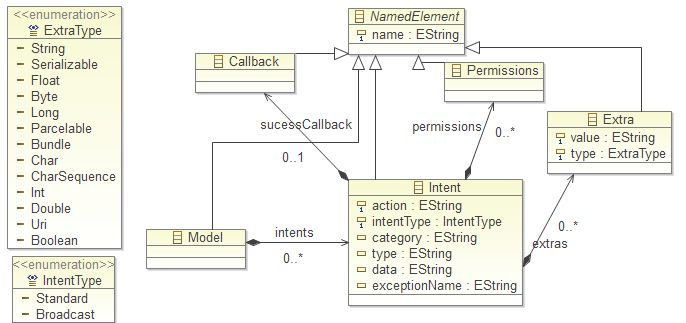
\includegraphics[width=\textwidth]{metamodel}
  \caption{Meta-model of Intent}
\end{figure}

The second stage of development was to take this model and build the Xtext grammar. The final Xtext grammar we produced was based on the default grammar that was generated but with several modifications for simplification and the use of enumerated types. To test the grammar we developed several models based on some examples that we had previously chosen. This allowed us to make changes to both the Xtext grammar and the Ecore model when one or both did not suit the required data from the Intents. The developed models in our DSL are used as our dataset for the plug-in. An example of an Intent in our DSL is shown below:

{\footnotesize\begin{lstlisting}[escapechar=!]
ImplicitIntent ActionSendText {
	type "text/plain"
	category "android.intent.category.DEFAULT"
	action "android.intent.action.SEND"
	extras {
		StringExtra "android.intent.extra.TEXT" !$\hookleftarrow$!
		"Put your text here"
	}
},
\end{lstlisting}}

The plug-in uses Model-to-Model transformations, and for this purpose we use JDT and AST as explained in the Section \ref{tools}. The dataset as defined in our abstract syntax is loaded, and the plug-in interface is built by iterating over the dataset; the final plug-in interface is presented in the figure \ref{codegeneratorview}. The interface allows a user to choose an Intent and generate the respective code in place where the cursor is. This code is generated through a Model-to-Model transformation from the data held in the abstract syntax to the AST nodes.

The plug-in is capable of handling the three different types of Intent identified; standard Activity Intents, broadcast Intents, and finally Intents with a callback. The plug-in provides several additional features to aid the developer: searching the dataset, enabling exception handling, producing callback methods if required, and finally the AndroidManifest.xml file is modified with any required permissions.


\begin{figure}[H]
\label{codegeneratorview}
  \centering
    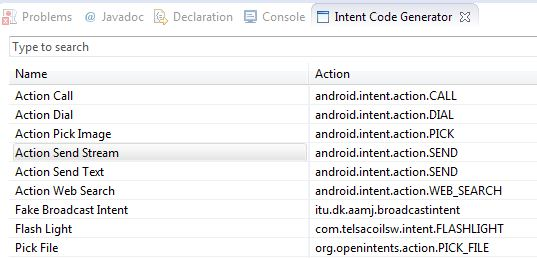
\includegraphics[width=\textwidth]{codegenerator}
  \caption{Code generator view}
\end{figure}

These additional features provide a quick and efficient experience for the developer, with intervention only required when the default settings produced should be modified.

Below we show an example of the generated code for an Intent which sends a customized text to a non specified receiver.

{\footnotesize\begin{lstlisting}
public class IntentExample
{
	private string text = "Hello World";
	int sendText(){
		Intent ast = new Intent("android.intent.action.SEND");
		ast.setType("text/plain");
		ast.putExtra("android.intent.extra.TEXT", text);
		startActivity(ast);		
	}
}
\end{lstlisting}}